\title{\Huge\textsf{\textbf{Convex Hull}}}
% \title{\Huge\textsf{\textbf{Convex Hull\\Report}}}
% \author{Paul Patault\thanks{\href{mailto:paul.patault@universite-paris-saclay.fr}{
%     \texttt{paul.patault@universite-paris-saclay.fr}}}\\
% \small Université Paris-Saclay}
\author{Paul Patault\\
\small Université Paris-Saclay}
\date{}
\documentclass[a4paper, 11pt]{article}

\usepackage[href, code]{ppbase}

\newcommand\question[2]{%
\medskip
\noindent{\color{blue}Question #1 : \textit{#2}}\\
}

\newcommand\qtt[1]{\texttt{\emph{#1}}}

\begin{document}

%%%%%%%%%%%%%%%%%%%%%%%%%%%%%%%%%%%%%%%%%%%%%%%%%%%%%%%%%%%%%%%%%%%%%%%%%%%%%%%
%%%%%%%%%%%%%%%%%%%%%%%%%%%%%%%%%%%%%%%%%%%%%%%%%%%%%%%%%%%%%%%%%%%%%%%%%%%%%%%

\thispagestyle{empty}
% \sffamily

\maketitle

\begin{abstract}
    The Jarvis algorithm is one way to solve the convex hull problem.
    I propose a formal specification of the problem and an implementation
    of this algorithm in the WhyML language with the aim to prove its correctness
    and termination.
\end{abstract}

%%%%%%%%%%%%%%%%%%%%%%%%%%%%%%%%%%%%%%%%%%%%%%%%%%%%%%%%%%%%%%%%%%%%%%%%%%%%%%
%%%%%%%%%%%%%%%%%%%%%%%%%%%%%%%%%%%%%%%%%%%%%%%%%%%%%%%%%%%%%%%%%%%%%%%%%%%%%%

\subsection*{Module \texttt{Point}}

\question{1}
    {Fill in the definition of the program function
    \qtt{lowest\_leftmost} of module \qtt{Point}, that compute the index
    of the lowest-leftmost point of a set.}

The function \texttt{lowest\_leftmost} searches for the “lowest” and “leftmost”
point in a set, according to the $y$ and $x$ projection, respectively. It will
be the initial point for the calculation of the convex hull. To identify it, I
just have to iterate through every point and remember the lowest-leftmost seen.
The contract of the function is

\begin{lstlisting}[language=whyml, escapechar=€, style=mystyle]
let lowest_leftmost (s:pt_set) : int
  requires { s.length > 0 }
  ensures  { is_index result s }
  ensures  { forall i: int. is_index i s -> is_lower_pt s[result] s[i] }
\end{lstlisting}

The post-conditions are given, I only add the pre-condition
in order to allow the access to the first element of the array \texttt{s}.
Then to prove this contact, I add some loop invariants :
(1) the current result is indeed the lowest-leftmost point,
(2) the result is a correct index of \texttt{s},
and (3) the memorized index corresponds to the lowest-leftmost
point found up to the current loop tour.

\begin{lstlisting}[language=whyml, escapechar=€, style=mystyle]
invariant { forall j: int. 0 <= j < i -> is_lower_pt s[r] s[j] }
invariant { is_index r s }
invariant { s[r] = rp }
\end{lstlisting}

It is quite trivial that all three are initially true, and preserved by the function.

\subsection*{Module \texttt{CCW}}

\question{2}
    {Complete the definition of the predicate \qtt{all\_on\_left(s,i,j)} that
    states that all the points from the point set \qtt{s}, distinct from
    \qtt{s[i]} and \qtt{s[j]}, are located to the left of the segment
    \qtt{s[i]}, \qtt{s[j]}. }

Let the function \texttt{diff2} which I will need and use later in the project%
\footnote{ One could think that we also need to check that \texttt{s[k] <>
    s[i]} and \texttt{s[k] <> s[j]} but it is not required. The situation where
    two points of \texttt{s} are equal is never happening, thanks to the assumption
    \texttt{no\_colinear\_triple}. Indeed,
    given that every pairwise points are colinear,
    and that a point \texttt{p$_1$} and its clone \texttt{p$_{1'}$}
    with the same coordinates are colinear,
    a colinear triple can be formed by selecting any other point in the set,
    which is a contradiction.}.

Using it to write the asked predicate gives the following

\begin{lstlisting}[language=whyml, escapechar=€, style=mystyle]
let function diff2 (k i j: int) : bool
= k <> i && k <> j

predicate all_on_left (s:pt_set) (i j:int)
= forall k: int.
    is_index i s ->
    is_index j s ->
    is_index k s ->
    diff2 k i j ->
    ccw s[i] s[j] s[k]
\end{lstlisting}

The predicate states as intended that all points of \texttt{s} are located on the left of
the \texttt{s[i]-s[j]} segment. Indeed, I must have for all \texttt{k} in \texttt{[0..length s - 1]}
% the \texttt{s[i]s[j]} segment. Indeed, I must have for all \texttt{k} in $[0..\text{length}(\texttt{s})-1]$
different from \texttt{i} and \texttt{j}, a “ccw-triangle” \texttt{s[i]s[j]s[k]}.

\question{3}
    {Complete the definition of the program function \qtt{check\_all\_on\_left}
    that decides whether \qtt{all\_on\_left(c, i, j)} holds. Notice that it is on
    purpose that this function does not return a Boolean but instead raises the
    exception \qtt{Exit} when the \qtt{all\_on\_left} predicate does not hold.}

The function \texttt{check\_all\_on\_left} can be written as

\begin{lstlisting}[language=whyml, escapechar=€, style=mystyle]
let check_all_on_left (s:pt_set) (i j:int) : unit
= for k = 0 to s.length - 1 do
    if diff2 k i j && not ccw s[i] s[j] s[k] then raise Exit
  done
\end{lstlisting}

with the following contract

\hfill

\pagebreak

\begin{lstlisting}[language=whyml, escapechar=€, style=mystyle]
let check_all_on_left (s:pt_set) (i j:int) : unit
  requires { is_index i s }
  requires { is_index j s }
  ensures  { all_on_left s i j }
  raises   { Exit -> not (all_on_left s i j) }
\end{lstlisting}

which expresses exactly what I want: given valid indices, we
ensure that all points of \texttt{s} are on the left of the
segment \texttt{s[i]s[j]}. Finally, I add the exceptional post-condition: if
\texttt{Exit} is raised then it should not be true that all points of
\texttt{s} are on the left of the segment \texttt{s[i]s[j]}.

To prove this specification correct and corresponding to the code, I only
need next invariant to be attached to the \texttt{for} loop.
\begin{lstlisting}[language=whyml, escapechar=€, style=mystyle]
invariant {
    forall l: int. 0 <= l < k -> diff2 l i j -> ccw s[i] s[j] s[l] }
\end{lstlisting}

It is required and enough to prove the post-condition.
Initially true because $\texttt{k} = 0$ (thus the range is null) and
preserved since as long as \texttt{Exit} is not raised then the test of the
\texttt{if} statement was evaluated to false.

\subsubsection*{Module \texttt{Path}}

Remark: I move the signature
\texttt{{\color{thered}val} nth(...)} to
\texttt{{\color{thered}val function} nth(...)} in order to
use it in the specifications.


\subsubsection*{Module \texttt{ConvexHull}}

\question{4}
    {Define a predicate \qtt{is\_convex\_hull(s,p)} that states that the path
    \qtt{p} is a convex hull of the point set \qtt{s}. This definition
    should make use of the predicate \qtt{all\_on\_left}. Justify carefully
    in your report why you pretend that your definition captures faithfully
    the notion of convex hull. For simplicity, to avoid degenerated cases,
    you may assume that considered sets of points have a minimal number of
    elements, say 2 or 3 (explain your choice in your report)}

First, I implement a program function of the given predicate distinct from
the following signature
\begin{lstlisting}[language=whyml, escapechar=€, style=mystyle]
let distinct (p:path) : bool
  ensures { result <-> distinct p }
= €$\ldots$€
\end{lstlisting}

With the help of this auxiliary function I was able to define
\texttt{wf\_path}, another auxiliary function implementing the
predicate \texttt{wf} defined as

\begin{lstlisting}[language=whyml, escapechar=€, style=mystyle]
predicate wf (p: path) (s: pt_set)
= distinct p /\
  forall i: int. is_valid_index i p -> is_index (nth p i) s
\end{lstlisting}

The proofs of the two last functions are quite simple. It is just necessary to
add some invariants to the \texttt{for} loops which are copy-paste of the
post-conditions bounded with respect to the current loop index.

In the end, the predicate \texttt{is\_convex\_hull} can be formulated as

\begin{lstlisting}[language=whyml, escapechar=€, style=mystyle]
predicate is_convex_hull (s:pt_set) (p:path)
= s.length >= __MIN_PTS_NUM__ /\
  wf p s /\
  (forall i: int. is_valid_index i p ->
    let j = if i+1 = p.size then 0 else i+1 in
    all_on_left s (nth p i) (nth p j))
\end{lstlisting}

\newcommand\ttp{\texttt{p}}

As suggested in the subject, I declared a constant
\texttt{\_\_MIN\_PTS\_NUM\_\_ = 2} to avoid degenerated cases. I choose 2 over
3 because only two points are required to be able to form one segment of the
path and this was the only limitation implied by the set cardinal. I will now
argue that the definition I choose for this predicate is what we want.
\begin{itemize}
    \item
        First I ask for the set \texttt{s} to be at least composed of two
        elements.
    \item
        The second condition to be a convex hull of a set \texttt{s} is to be a
        subset of \texttt{s}. This is exactly what I ask with the predicate
        \texttt{wf p s}: all elements of the path \texttt{p} must be unique (set property)
        and must be a valid index in the set \texttt{s} (subset property).
    \item
        Finally, I want to specify the following idea
        “if $X$ follows the path plotted by the points of \texttt{p},
        then every point of \texttt{s}
        (except for the two points between which $X$ moves)
        must be on $X$'s left”. Formally, for all pairs of consecutive points
        {\ttp'} and {\ttp''} in \texttt{p}
        (i.e (\ttp$_0$,\ttp$_1$) \cdots (\ttp$_{|p|-1}$,\ttp$_0$))
        the predicate \texttt{all\_on\_left s {\ttp'} {\ttp''}} must hold.
\end{itemize}

This definition seems to be complete when put in parallel to the description given
in the subject and the usual definition of a convex hull.

\question{5}
    {Complete the definition of the program function
    \qtt{check\_is\_convex\_hull} that, given a set of points and a path,
    decides whether the path describes the convex hull of the point set.
    This function must return a Boolean value, and it should make use of
    the function \qtt{check\_all\_on\_left}.}


The program function \texttt{check\_is\_convex\_hull} can be defined as follows

\begin{lstlisting}[language=whyml, escapechar=€, style=mystyle]
let check_is_convex_hull (s:pt_set) (p:path) : bool
  requires { s.length >= __MIN_PTS_NUM__ }
  ensures  { result <-> is_convex_hull s p }
=
  if not wf_path p s then False else
  try
    for i = 0 to p.size - 1 do
      let j = plus1mod i p.size in
      check_all_on_left s (nth p i) (nth p j)
    done;
    True
  with Exit -> False end
\end{lstlisting}

As intended, the only pre-condition is about the minimum cardinal of the point
set, while the post-condition is the equivalence between
\texttt{result} and \texttt{is\_convex\_hull s p}. That is, there are two
cases to consider, given by case analysis over the result of \texttt{wf\_path p
s}. In the first case, if it is false then we don't have a convex hull and we're
done. In the opposite, we can assume the predicate \texttt{wf p s}. Then we
only need to check that for every segment formed by a consecutive pair of
points in the path, it is the right extremity of the point set --- or more
explicitly, we must verify that all points are on the left of this segment.
If it is verified by all pairs of \texttt{p} then we have a proper convex hull,
otherwise we do not.

To prove this function correct, the invariant required
\begin{lstlisting}[language=whyml, escapechar=€, style=mystyle]
invariant {
  forall j: int. 0 <= j < i ->
    all_on_left s (nth p j) (nth p (plus1mod j p.size)) }
\end{lstlisting}
\noindent
is as usual a rewriting of the post-condition, bounded by the current index of
the \texttt{for} loop.

\question{6}
    {Prove the function \qtt{jarvis\_no\_termination} (a version
    ignoring termination), in the same time as developing the
    appropriate specification for largest.}


I added the following clauses to the contract of the \texttt{jarvis\_no\_termination} function.

\begin{lstlisting}[language=whyml, escapechar=€, style=mystyle]
let jarvis_no_termination (s:pt_set) : path
  requires { no_colinear_triple s }
  requires { exists i: int. unique_minimal_y s i }
  requires { length s >= __MIN_PTS_NUM__ }
  diverges
  ensures  { is_convex_hull s result }
= €$\ldots$€
\end{lstlisting}

The post-condition was given, also with the \texttt{diverges} option because we
are not interested into proving termination for now. The idea of this algorithm
is to gradually find the points of the path. Starting from the lowest-leftmost
point and performing a windscreen wiper movement, we can find the next point of
the path. Using the transitivity lemma, we know that we have to search for the
point maximizing the given relation.

Pre-conditions clauses are induced by the subject. As above we make a statement about
the size of the point set, and we add two more lemmas about this set for simplicity.
The first one claim that there are no triplets of colinear points, and the second
that there is exactly one lowest-leftmost point.

In order to prove this specification, I used the following invariants
\begin{lstlisting}[language=whyml, escapechar=€, style=mystyle]
invariant { is_index pivot s }                         (* 1 *)
invariant { is_index oldpivot s }                      (* 2 *)
invariant { p.size > 0 }                               (* 3 *)
invariant { nth p 0 <> pivot }                         (* 4 *)
invariant { nth p 0 = hd }                             (* 5 *)
invariant { nth p (p.size - 1) = pivot }               (* 6 *)
invariant { nth p (p.size - 2) = oldpivot }            (* 7 *)
invariant {
  forall i: int. 0 < i < p.size - 1 ->
    nth p i = pivot ->
    is_on_right s hd (nth p (i-1)) pivot }             (* 8 *)
invariant {
  forall i: int. 1 <= i < p.size ->
    all_on_left s (nth p (i-1)) (nth p i) }            (* 9 *)
invariant {
  forall i: int. 0 < i < p.size - 1 ->
    nth p i <> pivot }                                 (* 10 *)
invariant {
  forall i j: int.
    is_valid_index i p ->
    is_valid_index j p ->
    i < j ->
    nth p i <> nth p j }                               (* 11 *)
invariant { wf p s }                                   (* 12 *)
\end{lstlisting}

Invariants n°$[1,2]$ ensure the access to the corresponding elements of the
point set \texttt{s}. Invariant n°3 acts as a reminder to the system that
before the loop the path {\ttp} was not empty, and will never be. The following
four invariants n°$[4..7]$ state how the path is arranged.
The first element of the latter is different from \texttt{pivot} but equal to \texttt{hd}.
The last two elements are, following the order in which they were added, \texttt{oldpivot}
and \texttt{pivot}.
Invariants n°[4,5] are preserved because
the path never mutates and invariants n°[6,7] are derived from the inner code
of the \texttt{while} loop.


Invariants n°$[8, 10]$ are used to show that we cannot find any point more
than one time on the path. Let's have an in depth look at them.

A duplicated element is necessarily equal to the pivot when it has just been
added. That is, I claim that if one can find two times the pivot in the path,
then there is a duplicated element. The situation is the following: there is a
path of length \texttt{p.size}, starting by the point \texttt{hd}, and ending
with a loop linked by the pivot. By contradiction, we show that this situation
cannot happen. Indeed, the point \texttt{hd} (labeled \textsf{A} in the
following figure) would be on the right side of the segment \textsf{BC} where
\textsf{C} is \texttt{s[pivot]}. In this situation the function
\texttt{largest} should have returned the point \texttt{hd}. The property
\texttt{distinct p} is thus true.

\begin{figure}[h]
    \centering
    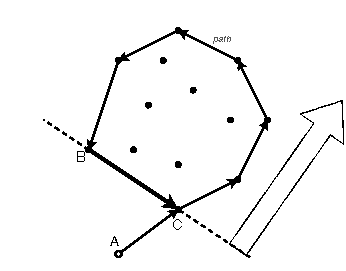
\includegraphics[scale=1.2]{./diag.drawio2.pdf}
    \caption{Intuition of the proof. \\
        {\small
    The point \textsf{A} is the “lowest-leftmost” point of the set, the big arrow
    shows the orientation of the left side of the last segment \textsf{BC} (in bold).} }
\end{figure}

Invariant n°11 verifies the injectivity of the function \texttt{nth p}.
Finally invariant n°12 is required to prove the post-condition.
It checks that the current path is well-formed, in accordance with the definition of the
\texttt{wf} predicate. It uses the 9th invariant and \texttt{distinct p} fact implied by
invariants n°[8,10] to be proved.

\pagebreak
\question{7}
   {Prove correct the function \texttt{largest}.}

The function \texttt{largest} can be specified with

\begin{lstlisting}[language=whyml, escapechar=€, style=mystyle]
let function largest (s: pt_set) (pivot: int) (ghost base: pt): int
  requires { no_colinear_triple s }
  requires { length s >= __MIN_PTS_NUM__ }
  requires { is_index pivot s }
  requires {
    forall k : int. is_index k s -> k <> pivot -> s[k] <> base ->
      ccw base s[pivot] s[k] }
  ensures { is_index result s }
  ensures { result <> pivot }
  ensures { all_on_left s pivot result }
=
  let ref res = if pivot = 0 then 1 else 0 in
  for i = res+1 to s.length - 1 do
    if i <> pivot then
      if ccw s[pivot] s[i] s[res] then
        res <- i;
  done;
  res
\end{lstlisting}


The first two requirements are the same as the function \texttt{jarvis}.
The next one is required to access to \texttt{s[pivot]} in the loop.
The last one is an invariant of the \texttt{jarvis} loop and is useful to know that
the pivot is the index in \texttt{s} of an element of the path.
The first post-condition ensures that the \texttt{result} is in \texttt{s},
the second that it is different from \texttt{pivot}
--- otherwise we could not ensure the strict progress of the path ---,
the third is the main requested property of the function.

The specification is provable with the following invariants

\begin{lstlisting}[language=whyml, escapechar=€, style=mystyle]
invariant { is_index res s }                           (* 1 *)
invariant { is_index (i-1) s }                         (* 2 *)
invariant { res <> pivot }                             (* 3 *)
invariant {
  forall j: int. 0 <= j < i ->
    diff2 j pivot res ->
    ccw s[pivot] s[res] s[j] }                         (* 4 *)
\end{lstlisting}

Invariants n°[1,2] are needed to access to \texttt{s} and they are trivially true.
Invariant n°3 proves the second to last post-conditions.
Obviously it is initially true and preserved thanks to the presence of the
\texttt{if} statements.
Finally invariant n°4 is initially true and preserved by the same \texttt{if} conditions.

\pagebreak
\question{8}
    {Prove the termination of the jarvis function. Any lemma or ghost
    function used must be proved too, including the inverse function
    if you use it.}

The patch to apply to the function \texttt{jarvis\_no\_termination} to prove
its termination is the following variant

\begin{lstlisting}[language=whyml, escapechar=€, style=mystyle]
variant { s.length - p.size }
\end{lstlisting}

I also need to use the two predicate given

\begin{lstlisting}[language=whyml, escapechar=€, style=mystyle]
predicate range (f: int -> int) (n: int) (m:int) =
    forall i: int. 0 <= i < n -> 0 <= f i < m

predicate injective (f: int -> int) (n: int) =
    forall i j: int. 0 <= i < j < n -> f i <> f j
\end{lstlisting}

The first is only about the bounds of a function \texttt{f}.
I use it to restrict the length of the domain and co-domain of a function.
The predicate \texttt{injective} is the usual definition for a function \texttt{f}
over a bounded domain.

Finally the three main lemmas proving the variant of \texttt{jarvis} are

\begin{lstlisting}[language=whyml, escapechar=€, style=mystyle]
lemma wf_injection:
  forall p: path. forall s: pt_set.
  wf p s ->
    injective (nth p) p.size /\
    range (nth p) (p.size) (s.length)

use pigeon.Pigeonhole

lemma enough_drawer_for_my_socks:
  forall p: path. forall s: pt_set.
   range (nth p) (p.size) (s.length) /\
   injective (nth p) (p.size) ->
   s.length >= p.size
\end{lstlisting}

The first one “adds” the two facts in the invariants of \texttt{jarvis}
as there is already the predicate \texttt{wf} for the path.
The second lemma is taken from the standard library of Why3 and is used to prove
the last but not least lemma, I named \\
\centerline{\texttt{enough\_drawer\_for\_my\_socks}.}
Given the conjunction I just proved with \texttt{wf\_injection},
we deduce \texttt{s.length >= p.size}. It is the last requirement to prove the
variant. Indeed, as I stated before the invariant \texttt{p.size > 0} provides a
positive size of the path before the loop. In combination with the first post-condition
of \texttt{Path.append} stating that the size of \texttt{p} grows, the termination
problem is solved. To sum up, we have a strictly growing and bounded quantity:
necessarily \texttt{p.size} will reach \texttt{s.length} at some point,
if the \texttt{Exit} exception has not been raised before.
This concludes the proof of the termination of the jarvis algorithm.

\subsection*{Conclusion}

It was a good project to deepen Why3.
I really appreciated to discover in this card the proposed algorithm.
I have encountered different problems, in particular when reasoning by the
absurd was a way to prove properties.
At the beginning it was not natural to think about “negative” invariants,
but in the end I got the trick.
I also wanted to emphasize the personal satisfaction of seeing IDE's lights
turn green one after the other until everything is proven.
Finally, I tried to write this report in English with the aim of improving myself.
I hope it will be intelligible enough.

\end{document}
